\section{\secmodarith}
\label{sec_mod_arith}

Many applications of number theory use a new number system based on remainders (\fn{mod}), which we introduce in this section. 

%%%%%%%%%%%%%%%%%%%%%%%%%%%%%

\newcommand{\subnotlast}{Not Last Game}
\subsection{\subnotlast}
\label{sub_not_last}

%This puzzle is 1-2 Nim.

In this puzzle, we introduce a game. To play the game, you will need an opponent (another person) and a pile of small objects such as coins, poker chips, candies, dried beans, etc.

\begin{act}[Not Last Puzzle]
\label{act_not_last}

The \vocab{Not Last} game starts with a pile of coins and two players, A and B.  Player A removes one or two coins, their choice.  Then player B removes one or two coins, their choice.  Then A goes again and then B.  They continue alternating until all the coins have been removed. At each turn each player must remove one or two coins.  Whoever takes the last coin loses (\vocab{\emph{mis\`ere}}) and, thus, each player's goal is to be ``not last''.  

For example, suppose the game begins with a pile of seven coins.  I, as the first player (A), remove two coins leaving a pile of five coins.  My opponent (B) decides to remove only one coin, thus leaving a pile of four.  I remove one more coin, leaving a pile of three.  My opponent chuckles as she removes two coins, leaving me to remove the last coin.  I lose. 

We can summarize this series of moves in the diagram: $$ 7 \xrightarrow{A-2} 5 \xrightarrow{B-1} 4 \xrightarrow{A-1} 3 \xrightarrow{B-2} 1 \xrightarrow{A-1} 0 \text{ B wins}.$$

I wonder if there is a different strategy where I could win with seven coins.  In general, for a pile of $n$ coins, is there a strategy by which the first player (A) can definitely win?  We assume, as is the custom, that both players are fully knowledgeable about the game, equally clever, and driven to win.

    \begin{actpart}
        \item Play four rounds of Not Last with seven coins to get a sense of the game and list the diagram for each.
    
        \item As we often do, let's begin by looking at the smallest special cases.  When $n=1$ who wins: A or B? Explain and draw the diagram. 
    
        \item When $n=2$ is there a strategy for A to win? Explain and draw the diagram.
    
        \item Repeat for $n=3$.
    
        \item When $n=4$, there is no strategy A can use to win. Draw diagrams for each option (A takes one coin or A takes two coins) showing that B wins in either case.
    
        \item Before we try larger values of $n$, it is helpful to shift our perspective slightly. As we play the game with $n$ coins, suppose there are eventually $k$ coins left.  For the purpose of this puzzle, $k$ is a \vocab{losing position} if the player who goes next eventually loses and $k$ is a \vocab{winning position} if the player who goes next eventually wins.  Explain why $k=1$ is a losing position, but $k=2$ and $k=3$ are winning positions.
        
        \item Let's revisit the 4-coin game with this new perspective. If A takes one coin, then $k=3$ which is a winning position and B goes next, so B wins.  If A takes two coins instead, then $k=2$ which is also a position number and B goes next, so B wins.  We can draw the simpler diagram, using the $\implies$ arrow to indicate a set of moves with known outcome.
        $$ 4 \xrightarrow{A-1} 3 \implies \text{ B wins} \text{ \quad OR \quad } 4 \xrightarrow{A-2} 2 \implies \text{ B wins}.$$
        We have just learned that $k=4$ is a losing position. 
        Find a strategy by which A wins when $n = 5$.  Explain and draw the diagram. Hint: How can A leave B in a losing position?% YES, A takes 1.
        
        \item When $n = 6$, is there a strategy by which A wins?  Explain and draw the diagram.  Remember, A is trying to leave B in a losing position, and vice versa.% YES, A takes 2
        
        \item When $n = 7$, is there a strategy by which A wins?  Explain and draw the diagram. % NO, A takes 1 or 2, B starts 5 or 6 so B wins
        
        \item Make a table showing $n=1,2,3,\ldots, 10$ in the top row and the winner (A or B) for each starting number of $n$ coins in the bottom row.  Be sure you check that the answer is correct for yourself, but you are not expected to explain your reasoning here.  
        
        \item Who do you think wins if the game starts with $n = 100$ coins? Is $k=100$ a winning position or a losing position? % This pattern repeats: after two YES it's a NO because if I take 1 or 2 those are both YES for B which is NO for me.  B wins 1, 4, 7, 10, . . . ., 100.  NO
    \end{actpart}
\end{act}

%%%%%%%%%%%%%%%%%%%%%%%%%%%%%

\newcommand{\submod}{The Mod Clock}
\subsection{\submod}
\label{sub_mod_clock}

There is a way to visualize the remainder of $a$ \fn{mod} $n$. 

\begin{rem}[Mod Clock]
To find $a$ \fn{mod} $n$ when $n \ge 1$, imagine an $n$ hour ``clock'' with hours marked $0, 1, 2, \ldots, n-1$ hours.  To find the value of $a$ \fn{mod} $n$ when $a$ is positive, we count $a$ hours clockwise from $0$.  The end mark is $a$ \fn{mod} $n$.  When $a$ is negative, we instead count counterclockwise.   
\end{rem}

\begin{exam}[Evaluating \fn{mod} using the Mod Clock]
\label{exam_eval_mod_clock}
~
    \begin{apart}
        \item Use the 12-hour clock (marked $0,1, \ldots, 11$ instead of the usual $1,2, \ldots 12$) shown in \Cref{fig_mod12_clock} to calculate 20 \fn{mod} 12.
               
        \begin{soln}
            We start at 0 and count clockwise 20 hours: $$1,2,3,4,5,6,7,8,9,10, 11,0,1,2,3,4,5,6,7,8.$$
            Thus 20 \fn{mod} 12 = 8.
        \end{soln} 

        \begin{figure}[hbtp]
            \centering
            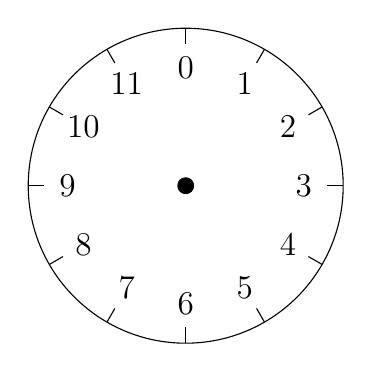
\begin{tikzpicture}
\node[circle,draw,minimum size=4cm] (a) at (0,0) {};
\filldraw (a.center) circle [radius=0.1cm];
\foreach \k in {0,1,...,11}
{
\draw (90-360/12*\k:1.8) -- (90-360/12*\k:2);
\draw (90-360/12*\k:1.5) node[font=\large] {\k};
}
\end{tikzpicture}

            \caption{The 12-hour clock}
            \label{fig_mod12_clock}
            \end{figure}
        
        \item Use the 5-hour clock shown in \Cref{fig_mod5_clock} to calculate 67 \fn{mod} 5.
            
        \begin{soln}
              Instead of counting off 67 hours, note that 50 hours will take us around the clock 10 times, ending at 0.  That leaves us $67-50-17$ hours to count from there.  Note that $15 = 3 \times 5$, so 15 hours will take us around the clock 3 times, ending at 0.  That leaves us $17-15 = 2$ hours to count from there, which ends at 2. Thus, 67 \fn{mod} 5 = 2.
         \end{soln}   

            \begin{figure}[ht]
            \centering
            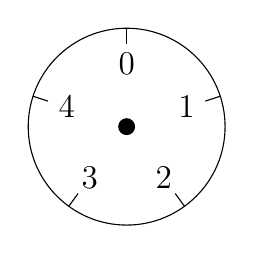
\begin{tikzpicture}
\node[circle,draw,minimum size=2.5cm] (a) at (0,0) {};
\filldraw (a.center) circle [radius=0.1cm];
\foreach \k in {0,1,...,4}
{
\draw (90-360/5*\k:1.05) -- (90-360/5*\k:1.25);
\draw (90-360/5*\k:0.8) node[font=\large] {\k};
}
\end{tikzpicture}

% \begin{tikzpicture}
% \node[circle,draw,minimum size=4cm] (a) at (0,0) {};
% \filldraw (a.center) circle [radius=0.1cm];
% \foreach \k in {0,1,...,4}
% {
% \draw (90-360/5*\k:1.8) -- (90-360/5*\k:2);
% \draw (90-360/5*\k:1.5) node[font=\large] {\k};
% }
% \end{tikzpicture}
            \caption{The 5-hour clock}
            \label{fig_mod5_clock}
            \end{figure}
            
        \item Use the 5-hour clock shown in \Cref{fig_mod5_clock} to calculate -12 \fn{mod} 5.
            \begin{soln}
                Since -12 is negative, we start at 0 count counterclockwise 12 hours:
                $$4,3,2,1,0,4,3,2,1,0,4,3.$$
                Thus, $-12$ \fn{mod} 5 = 3.
            \end{soln}
    \end{apart}
\end{exam}

Practice working with the mod clock.

\begin{act}[The Mod Clock]
\label{act_mod_clock} 
~
    \begin{actpart}
        \item Draw the 12-hour clock and use it to evaluate 17 \fn{mod} 12, 127 \fn{mod} 12, 4 \fn{mod} 12, and -2 \fn{mod} 12.
        \item Draw the 5-hour clock and use it to evaluate 17 \fn{mod} 5, 127 \fn{mod} 5, 4 \fn{mod} 5, and -2 \fn{mod} 5. 
    \end{actpart}
\end{act}

%%%%%%%%%%%%%%%%%%%%%%%%

\newcommand{\subzn}{The Integers mod $n$}
\subsection{\subzn}
\label{sub_integers_mod_n}

We can now define the integers mod $n$.

\begin{defn}[The integers mod $n$]
\label{defn_integers_modn}    
~
    \begin{apart}
        \item For a positive integer $n$, the \vocab{integers mod} $n$, denoted $\mathbb{Z}_n$ and pronounced ``Z mod $n$'', is the set 
            $$\mathbb{Z}_n = \{0, 1, 2,\ldots, n-1\}.$$
        For example,
            $$\mathbb{Z}_5 = \{0,1,2,3,4\}$$
        and
            $$\mathbb{Z}_{12} = \{0,1,2,3,4,5,6,7,8,9,10,11\}.$$

        \item We can define addition $\oplus$ and multiplication $\otimes$ on $\mathbb{Z}_n$ as follows:
            $$a \oplus b = (a+b)~\fn{mod}~n$$
            $$a \otimes b = (ab)~\fn{mod}~n$$
        For example, in $\mathbb{Z}_{10}$ , we have 
            $$5 \oplus 7 = 12~\fn{mod}~10 = 2,$$
            $$5 \otimes 7 = 35~\fn{mod}~10 = 5,$$  
        and $$4^2 = 4 \otimes 4 = 16 ~\fn{mod}~10 = 6.$$ 
        \item As in the usual order of operations (PEMDAS, \Cref{defn_integer_algebra_order_operations}, multiplication ($\otimes$) is higher priority than addition ($\oplus$).
        \item Addition and multiplication satisfy the \vocab{commutative property} $$a \oplus b = b \oplus a \text{ and } a \otimes b = b \otimes a,$$ the \vocab{associative property} $$(a \oplus b) \oplus c = a \oplus (b \oplus c) \text{ and } (a \otimes b) \otimes c = a \otimes (b \otimes c),$$ and the \vocab{distributive property} $$a \otimes (b \oplus c) = (a \otimes b) \oplus (a \otimes c).$$
    \end{apart}
\end{defn}

We can write arithmetic tables for $\mathbb{Z}_n$.

\begin{exam}[Addition and multiplication tables for $\mathbb{Z}_4$]
~
    \begin{apart}
        \item Write the addition and multiplication tables for $\mathbb{Z}_4$.
            \begin{soln}
                \Cref{table_mod4_arithm} shows the tables.  For example, $$1 \oplus 3 = 4~\fn{mod}~4 = 0$$ and $$2\otimes 3  = 6~\fn{mod}~4 = 2.$$
            \begin{table}[hbtp]
                \centering
                \begin{tabular}{ccc}
                    \begin{tabular} {l|llll} 
                        $\oplus$ & 0 & 1 & 2 & 3\\ \hline  
                        0 & 0 & 1 & 2 & 3\\ 
                        1 & 1 & 2 & 3 & 0 \\
                        2 & 2 & 3 & 0 & 1 \\ 
                        3 & 3 & 0 & 1 & 2 \\
                    \end{tabular}
                & ~\hspace{.5in}~ & 
                    \begin{tabular} {l|llll} 
                        $\otimes$ & 0 & 1 & 2 & 3 \\ \hline 
                        0 & 0 & 0 & 0 & 0\\
                        1 & 0 & 1 & 2 & 3\\ 
                        2 & 0 & 2 & 0 & 2\\ 
                        3 & 0 & 3 & 2 & 1\\ 
                    \end{tabular}
                \\
                \end{tabular}
                \caption{The arithmetic tables for $\mathbb{Z}_4$, the integers mod 4.}
                \label{table_mod4_arithm}
            \end{table}
            \end{soln}
        \item True or false?  If $a \otimes b = 0$ in $\mathbb{Z}_4$, then $a = 0$ or $b = 0$.
            \begin{soln}
                The question is asking if there are any 0s in the multiplication table other than in the row and column headed by 0.  It turns out there are and so this statement is false.  As a counterexample, $2 \neq 0$, but $2 \otimes 2 = 4~\fn{mod}~4= 0$ in $\mathbb{Z}_4$.
            \end{soln}
        \item For which values of $a \in \mathbb{Z}_{4}$, does $a \otimes x = 1$ have a solution? 
            \begin{soln}
                The question is asking which rows in the multiplication table have a one in them?  The rows headed by 1 and 3 each have a 1 because $1 \otimes 1 = 1$ and also $3 \otimes 3 = 1$.  The answer is $a = 1, 3$.  (It is coincidence that the corresponding solutions are $x=1, 3$.)
            \end{soln}
    \end{apart}
\end{exam}

It is your turn to work with arithmetic in the integers mod $n$.

\begin{act}[Arithmetic mod $n$]
\label{act_arith_modn}
~
    \begin{actpart}
        \item In $\mathbb{Z}_5$ confirm that $2 \oplus 4 = 1$ and $2 \otimes 4 = 3$.
        \item In $\mathbb{Z}_6$ confirm that $2 \oplus 4 = 0$ and $2 \otimes 4 = 2$.
        \item \label{part_arith_table_mod5_mod6} Write the addition and multiplication tables for $\mathbb{Z}_5$ and $\mathbb{Z}_6$.  Hint: If you are working with a partner, then one of you should do $\mathbb{Z}_5$ while the other does $\mathbb{Z}_6$, just check each other's work.  We need these tables for later parts of this activity.
        \item True or false?  If $a \otimes b = 0$ in $\mathbb{Z}_6$, then $a = 0$ or $b = 0$. What about in $\mathbb{Z}_5$?
        \item For which values of $a \in \mathbb{Z}_{5}$, does $a \otimes x = 1$ have a solution? What about in $\mathbb{Z}_6$?
    \end{actpart}
\end{act}

%%%%%%%%%%%%%%%%%%%%%%%%%%%%%%%%%%%%%%%%%%

\subsection{Exercises}

%%%%%%%%%%%%%%%%%%%%%%%%%%%%%%%%%%%%%%%%%%

\subsection*{Exercises for \Cref{sub_not_last} \subnotlast}

\begin{exer}[\exerP] % winning position Not Last
\label{exer_not_last_winning_position}
    This exercise refers to the Not Last game introduced in \Cref{act_not_last}.  We know that one and four are losing positions, whereas two and three are winning positions.
    \begin{exerpart}
            \item Explain why five is a winning position.
            \item Explain why six is a winning position.
            \item Explain why seven is a losing position.
    \end{exerpart}
\end{exer}

\begin{exer}[\exerU] % who wins Not Last?]
\label{exer_not_last_conj} 
    This exercise refers to the Not Last game introduced in \Cref{act_not_last}.  
        \begin{exerpart}
            \item Which integers $n$ are a losing position?  State your answer as a conjecture.  Hint: Use \fn{mod} in your answer. %A wins if $n \equiv 0 (mod 3)$ or $n \equiv 2 (mod 3)$. B wins when $n \equiv 1 (mod 3)$.
            \item Suppose that you are in a winning position $n$ while playing the Not Last game introduced in \Cref{act_not_last}.  What is your strategy for deciding whether to take one or two coins? Be specific. Hint: Your answer should involve $n$ and use \fn{mod}.
        \end{exerpart} 
\end{exer}

% \begin{exer}[\exerR] % Not last
% \label{exer_dyk_nim}
%     Do you know \ldots
%         \begin{exerpart}
%             \item 
%         \end{exerpart}
% \end{exer}

\begin{exer}[\exerE] % new Half game example]
\label{exer_half_game123}
    In this exercise we define a new game, \vocab{Half}, which starts with a pile of coins and two players, A and B.  Player A goes first and then A and B take turns removing coins from the pile.  The rule is that at each turn, a player must remove at least one coin and at most half of the coins, with the exception that if there is one coin left, then they must take it.  For example, if there are six or seven coins, the next player can take one, two, or three coins. As in the Not Last game, whoever takes the last coin loses the Half game.   
    \begin{exerpart}
        \item Who wins the Half game when $n=1,2,3$, the first player (A) or the second player (B)? Explain.% B wins 1, A wins 2 (take 1), B wins 3.
        \item Who wins the Half game when $n=4,5,6,7$?  Explain.  % A wins 4 (take 1), A wins 5 (take 2), A wins 6 (take 3), B wins 7 
    \end{exerpart} 
\end{exer}

\begin{exer}[\exerE] % who wins Half?]
\label{exer_half_conj}
    This exercise refers to the Half game introduced in \Cref{exer_half_game123}. Complete \Cref{exer_half_game123} before trying this exercise.
        \begin{exerpart}
            \item Which integers $n$ are a losing position in the Half game?  State your answer as a conjecture.  % B wins when $n$ is $2^k-1$ for some integer $k$.  Else A wins.
            \item Suppose that you are in a winning position $n$ while playing Half.  What is your strategy for deciding how many coins to take?  Hint: your answer should involve $n$.
            %Answer:  If possible, you want to remove coins to leave them at one less than a power of 2.  Say $2^k$ is the greatest power of 2 in n  (meaning $2^k \le n < 2^{k+1}$) and write $n = 2^k + r$ where $r< 2^k$. You want to leave them at $2^k-1$.  To do so, remove $r+1$ coins. Let's check that this is allowed.  Note that if $n =2^{k+1}-1$, then you lose. Else, we must have $n \le 2^{k+1}-2$ and so $n+2 \le 2^{k+1}$. Thus $$r+1 = n-2^k +1 = n - \frac{2^{k+1}}{2}+1 \le n - \frac{n+2}{2}+1 = \frac{2n-(n+2)+2}{2}= \frac{n}{2}$$ which is allowed.
        \end{exerpart}
\end{exer}

%%%%%%%%%%%%%%%%%%%%%%%%

\subsubsection*{Exercises for \Cref{sub_mod_clock}
\submod}

\begin{exer}[\exerP] %Using the mod clock
\label{exer_eval_mod_clock}
    In each part of this exercise, draw the relevant mod clock and show how to use it to evaluate the quantity.  Recall that we rotate clockwise for positive integers.
    \begin{exerpart}
        \item 23 \fn{mod} 5. Hint: Copy the mod 5 clock from \Cref{fig_mod5_clock}.
        \item 23 \fn{mod} 12. Hint: Copy the mod 12 clock from \Cref{fig_mod12_clock}.
        \item 23 \fn{mod} 10. Hint: The mod 10 clock has labels $0,1,2,3,4,5,6,7,8,9$.
        \item 23 \fn{mod} 6. Hint: The mod 6 clock has labels $0,1,2,3,4,5$.
    \end{exerpart}
\end{exer}

\begin{exer}[\exerU] % Negatives on mod clock
\label{exer_neg_mod_clock}
    In each part of this exercise, draw the relevant mod clock and show how to use it to evaluate the quantity.  Recall that we rotate counterclockwise for negative integers.
    \begin{exerpart}
        \item $-10$ \fn{mod} 5
        \item $-10$ \fn{mod} 6
        \item $-10$ \fn{mod} 12
        \item $-10$ \fn{mod} 3
    \end{exerpart}
\end{exer}

\begin{exer}[\exerR] % mod clock
\label{exer_dyk_mod_clock}
    Do you know \ldots
        \begin{exerpart}
            \item How to calculate $a~\fn{mod}~n$ using a ``mod clock''? Make sure your answer includes both positive and negative numbers $a$.
            \item What values of $a$ have $a~\fn{mod}~n=0$?  That is, which values of $a$ end at 0 on the \fn{mod} $n$ clock?
        \end{exerpart}
\end{exer}

\begin{exer}[\exerE] %name
%\label{exer_name}
~
    \begin{exerpart}
        \item Use the idea of a mod $n$ clock to explain why $a$ \fn{mod} $n=0$ whenever $a$ is a multiple of $n$.
        \item Use the idea of a mod $n$ clock to explain why $-1$ \fn{mod} $n=n-1$ and $-2$ \fn{mod} $n=n-2$.  Hint: The mod $n$ clock has labels $0,1,2,\ldots,n-1$.
    \end{exerpart}
\end{exer}

%%%%%%%%%%%%%%%%%%%%%%%%

\subsubsection*{Exercises for \Cref{sub_integers_mod_n}
\subzn}

\begin{exer}[\exerP] %tables mod 2 and mod 3.
\label{exer_arith_tables_mod2_mod3}
~
    \begin{exerpart}
        \item Write out the addition and multiplication tables for $\mathbb{Z}_3=\{0,1,2\}$.  Hint: Each entry in your tables should be 0, 1, or 2.
        \item Write out the addition and multiplication tables for $\mathbb{Z}_2=\{0,1\}$.  Hint: Each entry in your tables should be 0 or 1.
    \end{exerpart}
\end{exer}

\begin{exer}[\exerP] % arithmetic tables for $\mathbb{Z}_n$]
\label{exer_arith_table_mod5_mod6_again}
    This exercise repeats \Cref{act_arith_modn} (\ref{part_arith_table_mod5_mod6}).
        \begin{exerpart}
            \item Write out the arithmetic tables for $\mathbb{Z}_5$.
            \item Write out the arithmetic tables for $\mathbb{Z}_6$.  
    \end{exerpart}
\end{exer}

\begin{exer}[\exerU] %solve linear equations mod n
\label{exer_solve_linear_modn}
    For each equation, find every solution $\mathbb{Z}_n$, if any, by checking each element of $\mathbb{Z}_n$ to see if it is a solution.
        \begin{exerpart}
            \item Solve $x \oplus 4 = 1$ in $\mathbb{Z}_5$.  
            \item Solve $x \oplus 4 = 1$ in $\mathbb{Z}_6$.
            \item Solve $2 \otimes x = 3$ in $\mathbb{Z}_5$.
            \item Solve $2 \otimes x = 3$ in $\mathbb{Z}_6$.
            \item Solve $3 \otimes x \oplus 1 = 3$ in $\mathbb{Z}_5$.  Note that the usual order of operations applies, so this equation means $(3 \otimes x) \oplus 1 = 3$
        \end{exerpart}
\end{exer}

\begin{exer}[\exerU] % square root -1 examples
\label{exer_modn_sqrtminus1_examples}
    In $\mathbb{Z}_n$, we write $x^2=x \otimes x$.
    \begin{exerpart}
        \item  In $\mathbb{Z}_5$, what are the solutions, if any, of $x^2\oplus 1 = 0$?  
        \item  In $\mathbb{Z}_6$, what are the solutions, if any, of $x^2\oplus 1 = 0$? 
        \item  In $\mathbb{Z}_{10}$, what are the solutions, if any, of $x^2\oplus 1 = 0$? 
        \item In $\mathbb{Z}_2$, what are the solutions, if any, of $x^2\oplus 1 = 0$? 
    \end{exerpart}
\end{exer}

\begin{exer}[\exerU] % zero divisor mod n examples
\label{exer_zero_divisors_examples}
~
    \begin{exerpart}
        \item Give an example of elements $a$ and $b$ in $\mathbb{Z}_{10}$ where $a \otimes b = 0$, but $a \neq 0$ and $b \neq 0$.
        \item Can you find elements $a$ and $b$ in $\mathbb{Z}_5$ where $a \otimes b = 0$, but $a \neq 0$ and $b \neq 0$?  Explain.  
    \end{exerpart}
\end{exer}

\begin{exer}[\exerU] % units mod n examples
\label{exer_modn_units_examples}
~
    \begin{exerpart}
        \item  For which values of $a \in \mathbb{Z}_5$, does $a \otimes x = 1$ have a solution?  
        \item For which values of $a \in \mathbb{Z}_6$, does $a \otimes x = 1$ have a solution? 
        \item For which values of $a \in \mathbb{Z}_{10}$, does $a \otimes x = 1$ have a solution?  You should be able to answer without writing the multiplication table.
        \item For which values of $a \in \mathbb{Z}_8$, does $a \otimes x = 1$ have a solution?  You should be able to answer without writing the multiplication table.
    \end{exerpart}
\end{exer}

\begin{exer}[\exerR] % the integers mod n
\label{exer_dyk_integers_modn}
    Do you know \ldots
        \begin{exerpart}
            \item What $\mathbb{Z}_n$ is?
            \item How to add and multiply in the integers mod $n$?
            \item How to construct the addition and multiplication tables mod $n$.
            \item How to solve equations in $\mathbb{Z}_n$? 
        \end{exerpart}
\end{exer}

\begin{exer}[\exerE] % powers mod n examples
\label{exer_powers_modn_examples}
    In $\mathbb{Z}_n$, we write $2^k=\underbrace{2 \otimes 2 \otimes 2 \otimes \cdots \otimes 2}_{k \text{ times}}.$  On this exercise, you are welcome to use computational technology.
        \begin{apart}
            \item \label{part_powers2_mod5} In $\mathbb{Z}_5$, calculate $2^1$, $2^2$, $2^3$, $2^4$, $2^5$, $2^6$, $2^7$, and $2^8$.  
            % Hint: For example, because $2^3=8 \fn{ mod } 5 = 3$, it follows that
            %     \begin{align*}
            %         2^4 \fn{ mod } 5 &= (2 \otimes 2^3) \fn{ mod } 5 \\
            %         & = (2 \otimes 8) \fn{ mod } 5 \\
            %         & = (2 \otimes 3) \fn{ mod } 5 \\
            %         & = 6 \fn{ mod } 5 \\
            %         & = 1.
            %     \end{align*}
            % That is, you can calculate each power from the previous power by multiplying by two and then reducing mod. For example, 
            %     \begin{align*}
            %         2^5 \fn{ mod } 5 & = (2 \otimes 2^4) \fn{ mod } 5 \\
            %         & =(2 \otimes 1) \fn{ mod } 5  \\
            %         & = 2.
            %     \end{align*}

            \item Based on the pattern in (\ref{part_powers2_mod5}), conjecture the value of $2^{50}$. Explain your reasoning.
            \item \label{part_powers2_mod6} In $\mathbb{Z}_6$, calculate $2^1$, $2^2$, $2^3$, $2^4$, $2^5$, $2^6$, $2^7$, and $2^8$.  
            \item Based on the pattern in (\ref{part_powers2_mod6}), conjecture the value of $2^{50}$.Explain your reasoning.
        \end{apart}
\end{exer}

\begin{exer}[\exerE] % zero divisors mod n conjecture
\label{exer_zero_div_modn_conj}  
~
    An element $a$ of $\mathbb{Z}_n$ is a \vocab{zero divisor} if $a \neq 0$ but there is an element $b$ of $\mathbb{Z}_n$ with $b \neq 0$ also, and yet $ab = 0$. That is, if there is more than one 0 in the row for $a$ in the multiplication table for $\mathbb{Z}_n$. \Cref{exer_zero_divisors_examples} asked for an example of a zero divisor in $\mathbb{Z}_{10}$ and asked whether there were zero divisors in $\mathbb{Z}_5$.  Conjecture which integers $n$ have the property that $\mathbb{Z}_n$ has zero divisors and which integers $n$ have the property that $\mathbb{Z}_n$ does not have zero divisors.
    %% SU:  foreshadow prime and composite.  Could circle back (or not).
\end{exer}

%%%%%%%%%%%%%%%%%%%%%%%%%%%
\subsection{\answers}
%%%%%%%%%%%%%%%%%%%%%%%%%%%

%%%%%%%%%%%%%%%%%%%%%%%%%%%%%%%%%%%%%%%%%
\subsubsection{\answers for \Cref{sub_not_last} \subnotlast}

\subsubsection*{\Cref{exer_not_last_winning_position} \answers}
\begin{apart}
    \item Take one to leave your opponent with four, which is a losing position.
    \item Hint: You want to leave your opponent in four again.
    \item Hint: Consider the two cases where one or two is taken.
\end{apart}

\subsubsection*{\Cref{exer_not_last_conj} \answers}
\begin{apart}
    \item Hint: Your answer depends on \fn{mod} 3.
    \item Hint: Look at $n \fn{ mod } 3$ and break down your answer into cases.
\end{apart}

%%%%%%%%%%%%%%%%%%%%%%%%
\subsubsection{\answers for \Cref{sub_mod_clock}
\submod}

\subsubsection*{\Cref{exer_eval_mod_clock} \answers}
  The answers in some order are zero, one, three, and five.

\subsubsection*{\Cref{exer_neg_mod_clock} \answers}
    The answers to each part are zero or two.
    
%%%%%%%%%%%%%%%%%%%%%%%%
\subsubsection{\answers for \Cref{sub_integers_mod_n} \subzn}

\subsubsection*{\Cref{exer_arith_tables_mod2_mod3} \answers}
\begin{apart}
    \item Hint: Check that $2 \oplus 2 = 1$ and $2 \otimes 2 = 1$.
    \item Hint: The only unusual entry is $1 \oplus 1 = 0$.
\end{apart}

\subsubsection*{\Cref{exer_arith_table_mod5_mod6_again} \answers}
\begin{apart}
    \item Hint: The rows for two are $2,4,1,3,0$ and $0,2,4,3,1$.
    \item Hint: The rows for two are $2,4,0,2,4,0$ and $0,2,4,0,2,4$.
\end{apart}

\subsubsection*{\Cref{exer_solve_linear_modn} \answers}
\begin{apart}
    \item $x=2$
    \item Hint: There is one solution.
    \item $x=4$
    \item Hint: Look at the row for two in the multiplication table. Explain why there is no solution.
\end{apart}

\subsubsection*{\Cref{exer_modn_sqrtminus1_examples} \answers}
\begin{apart}
    \item Hint: Two of $0,1,2,3,4$ are solutions.  Check each one.
    \item Hint: There is no solution.
    \item Hint: One solution is $x=3$. There is a second solution.
    \item Hint: There is one solution.
\end{apart}

\subsubsection*{\Cref{exer_modn_units_examples} \answers}
\begin{apart}
    \item $a=1,2,3,4$
    \item Hint: $a=1$ and one more value.  Look for ones in the multiplication table.
    \item Hint: There are four values of $a$, all odd.
    \item $a=1,3,5,7$
\end{apart}

\subsubsection*{\Cref{exer_powers_modn_examples} \answers}
\begin{apart}
    \item Hint: The list begins $2, 4, 3, \ldots$.
    \item Hint: The list begins $2,4,2,\ldots$.
\end{apart}


